\section{Experiments}
\subsection{Datasets}
We also evaluate the performance based on the most typical benchmark on real datasets:
the quantitative structure-activity relationship (QSAR). 
We select Four binary-classification datasets (CPDB, Mutag, AIDS(CAvsCM), CAS) in Table~\ref{tbl:dataset}: 
CPDB and Mutag for mutagenicity tests and AIDS(CAvsCM) for antiviral tests.
All chemical structures are encoded as molecular graphs using RDKit\footnote{\url{http://www.rdkit.org/}}, 
and some structures in the raw data are removed by chemical sanitization\footnote{
Due to this pre-processing, the number of datasets differs from that 
in the simple molecular graphs in the literature, 
where the nodes are labeled by atom type, and the edges are labeled by bond type.}.
We simply apply a node labeling by the RDKit default atom invariants (edges not labeled), i.e., 
atom type, \# of non-H neighbors, \# of Hs, charge, isotope, and inRing properties. 
These default atom invariants use connectivity information similar to that used for the well-known 
ECFP family of fingerprints\cite{Rogers:2010}. See \cite{Kearnes2016} for more elaborate encodings.

\tabcolsep = 6pt
\begin{table}[h]
  \centering
  \caption{Dataset summary}
  \label{tbl:dataset}
  	\begin{tabular}{lcccc}
		\thickhline
		Dataset			& CPDB           & Mutag        & AIDS(CAvsCM)     & CAS	\\  \hline
		\# data			& 684            & 188          & 1503             & 4337	\\
		\# ($y=+1,-1$)	& (341, 343)     & (125, 63)    & (422, 1081)      & (2401, 1936)	\\  
		\# nodes		& 25.2           & 26.3         & 59.0             & 30.3	\\  
		\# edges		& 25.6           & 28.1         & 61.6             & 31.3	\\  
		\thickhline
		\end{tabular}
  \leftline{\hspace*{2pt} \# of nodes and edges are average.}
\end{table}

\subsection{UNDER CONSTRUCTION}
\begin{figure}[htbp]
 \begin{minipage}{0.5\hsize}
  \begin{center}
   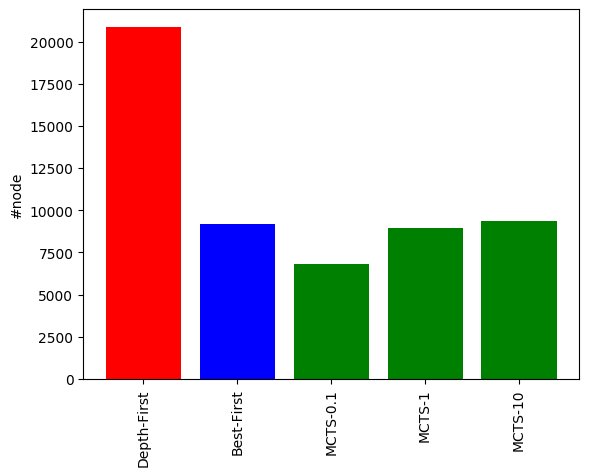
\includegraphics[width=60mm]{img/cas/artificial/1/node.png}
  \end{center}
  %\caption{一つめの図}
  \label{fig:one}
 \end{minipage}
 \begin{minipage}{0.5\hsize}
  \begin{center}
   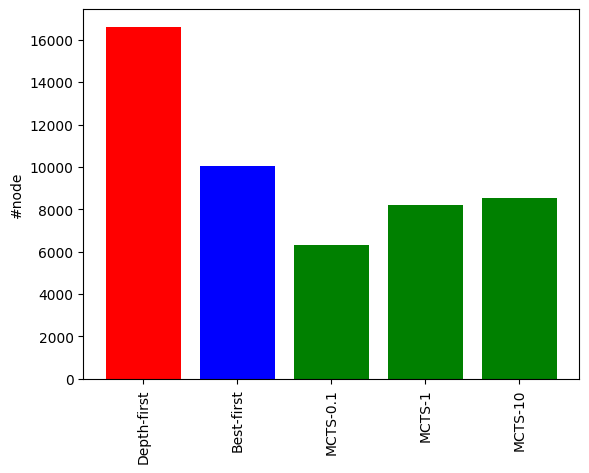
\includegraphics[width=60mm]{img/cas/artificial/2/node.png}
  \end{center}
  %\caption{二つめの図}
  \label{fig:two}
 \end{minipage}
 \caption{一つめの図}
\end{figure}

\begin{comment}
\subsection{MCTS Cost Performance Comparison to Exact Search}
\label{sec:experimentspeed}
As previously mentioned in Section~\ref{sec:relatedwork}, \ref{sec:ourapproach}, 
%our method is based on \cite{Shirakawa:2018} that search optimal feature exactly using tricky pruning, 
our method is based on that search optimal feature exactly using tricky pruning, 
in this section we call the previous method GTB-exact, and proposed method GTB-MCTS.

MCTS is able to control the cost of feature search by setting the number of Monte Carlo simulations.
We investigate the cost performance of MCTS and compare with previous exact method.
Each hyperparameters is shared(the number of trees: 100, max tree depth: 3, stepsize: 1.0) 
and MCTS specific parameters is fixed(exploration constant: 1).
In this experimental setup, AIDS(CAvsCM) is used 
and the maximum subgraph size of feature search space is set to 10.
Since GTB-MCTS has randomness in the model, 10 model averages and variance values are used for evaluation.
Fig~\ref{fig:costperformance} shows the model construction time, training loss, and test accuracy compared
among each cost GTB-MCTS(the number of Monte Carlo simulations = [10,100,200,300,400,500]) and GTB-exact.
The left figure is log-scale, and this shows the construction time of GTB-MCTS increases linearly 
with the number of Monte Carlo simulations.
The lower the search cost, the greater the training loss mean,
however the test accuracy is higher than GTB-exact at lower search cost.
For example, the GTB-MCTS(the number of Monte Carlo simulations = 100) is build the higher accuracy model 
about 100 times faster than GTB-exact.
It is interesting that the accuracy can be improved in spite of reducing the search cost.
Then we investigate the detail of the features used in these models.

Fig~\ref{fig:featuresize} shows the size ratio of the features used to learn the model.
We can observe that the features that GTB-exact uses for learning are almost big, 
about 80\% are subgraphs with 9 or 10 edges.
On the other hand, GTB-MCTS has a balanced features size ratio unless the search cost is too low.
Therefore, GTB-MCTS has higher generalization ability than GTB-exact, which led to improve the test accuracy.
\begin{figure}[t]
 \centering
  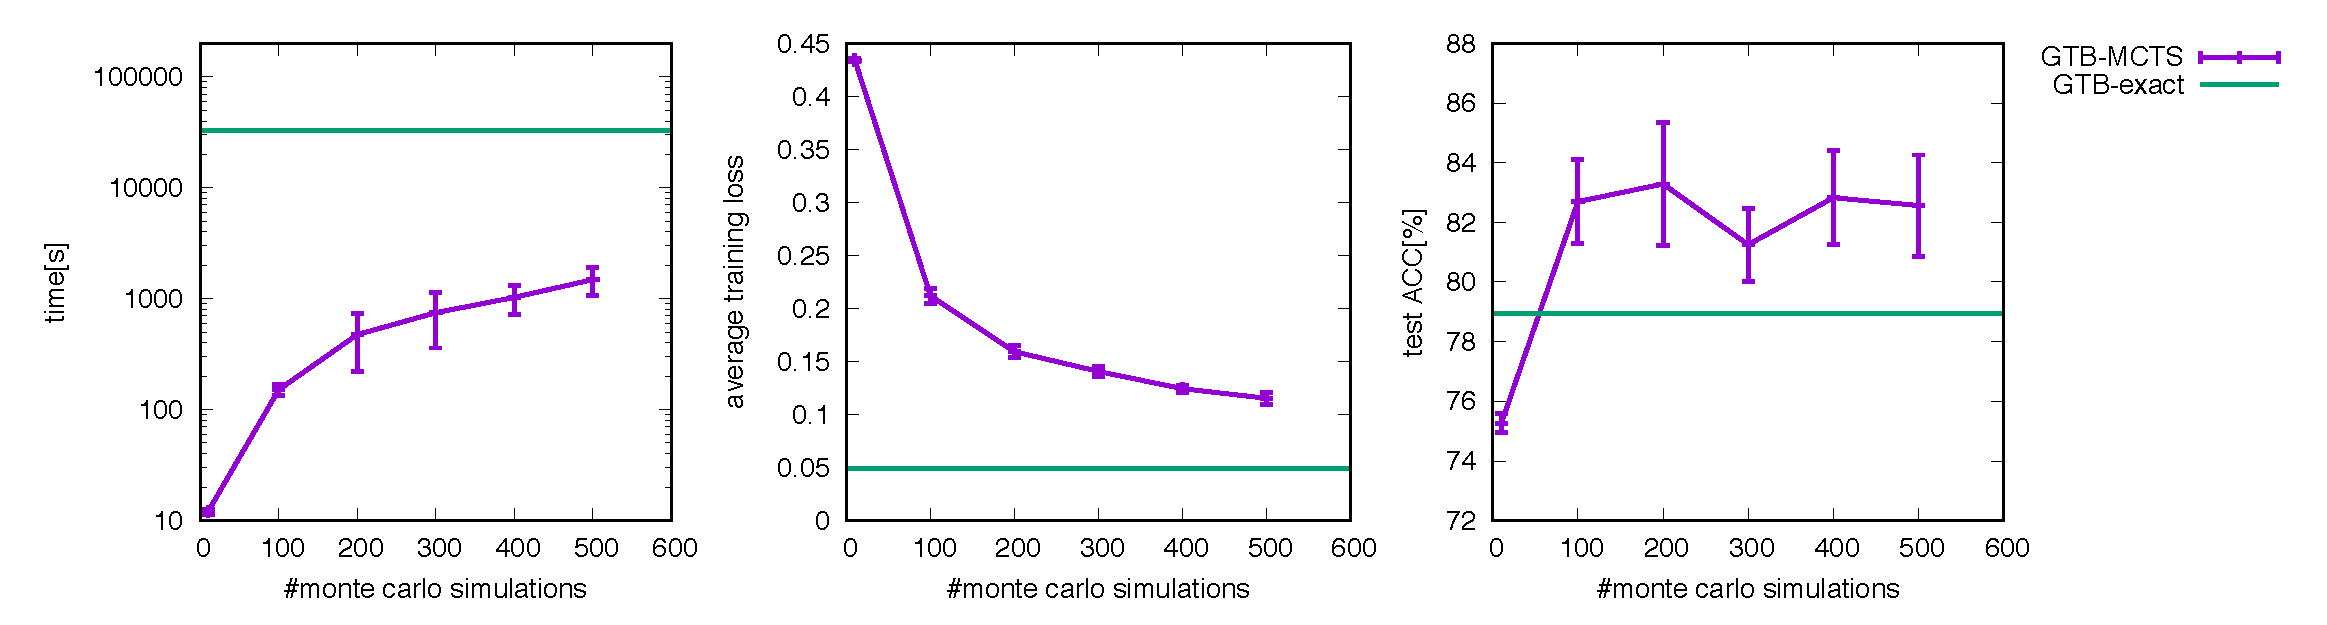
\includegraphics[width=1\textwidth]{img/speed.eps}
   \caption{Search cost performance}
   \label{fig:costperformance}
\end{figure}
\begin{figure}[t]
 \centering
  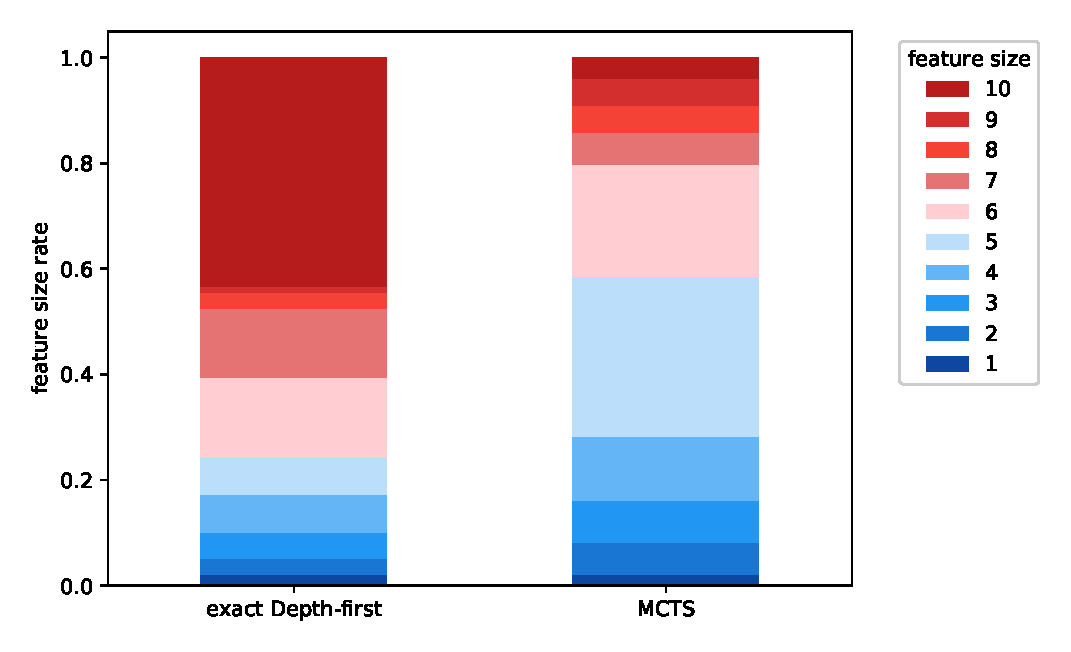
\includegraphics[width=0.55\textwidth]{img/feature_rate.eps}
   \caption{Features size ratio}
   \label{fig:featuresize}
\end{figure}

\subsection{Accuracy for the QSAR}
Tables~\ref{tbl:acc} shows the performance results obtained 
by 10-fold cross validations for QSAR datasets.
We use the same two nonlinear methods used before 
and one linear method, gBoost\cite{Saigo:2009} that is the basis of our method. 
The hyperparameter tuning is performed for the ranges described in Table~\ref{tbl:param}, 
and the best parameters are also listed in Table~\ref{tbl:bestParam}.
We can observe that nonlinear methods often outperform the linear method. 
At the same time, our proposed method GTB-MCTS achieves the best performance except for CPDB. 
The overall accuracy for the CPDB is also the second, 
this shows that our proposed method is able to be a good solution for real datasets.

\tabcolsep = 13pt
\begin{table}[t]
  \centering
  \caption{Hyperparameter settings for the QSAR}
  \label{tbl:param}
  \scalebox{0.85}{
   \begin{tabular}{llcl}
     \multicolumn{3}{l}{\textit{Common}} \\
     \thickhline
     %\multicolumn{2}{|l}{min support} & $m$(\%) & 10, 5, 2.5, 0 \\
     \multicolumn{2}{l}{max subgraph size (\# edges)} & $x$ & 4, 6, 8 \\
     \thickhline
     \multicolumn{3}{l}{} \\
     \multicolumn{3}{l}{\textit{Model specific}} \\
     \thickhline
     GTB- & max tree depth & $d$ & 1, 3, 5 \\
     (MCTS, exact) & stepsize & $\eta$ & 0.1, 0.4, 0.7, 1.0 \\
     ~ & \# trees & $k$ & 1-500 \\
     \hdashline[2pt/1pt]
     (MCTS) & \# monte carlo simulations & $i$ & 100, 300, 500 \\
     ~ & exploration constant & $c$ & 1, 10, 100 \\
     \hline
     gBoost & regularization & $\nu$ & {0.01, 0.1, 0.2, 0.3,}{0.4, 0.5, 0.6} \\
     \thickhline
   \end{tabular}
  }
\end{table}

\tabcolsep = 7pt
\begin{table*}[t]
  \centering
  \caption{Prediction accuracy (\%) for the QSAR}
  \label{tbl:acc}
  \scalebox{0.87}{
  	 \begin{tabular}{lcccccc}
  	   \thickhline
  	   ~								& CPDB						& ~							& Mutag						& ~							& AIDS(CAvsCM)						& ~ 						\\
  	   ~   							& ACC       				& AUC       				& ACC       				& AUC       				& ACC                 				& AUC              			\\ \hline
  	   \multicolumn{7}{l}{\textit{Nonlinear models}} \\
  	   \ss{GTB-MCTS}{~}                & \ss{79.0}{($\pm$2.7)}     & \ss{83.7}{($\pm$2.7)}     & \fss{91.0}{($\pm$5.0)}  	& \fss{94.8}{($\pm$5.0)}   	& \fss{84.4}{($\pm$2.8)}   			& \fss{85.3}{($\pm$2.8)}   	\\
  	   \ss{GTB-exact}{~}                		& \fss{80.3}{($\pm$4.5)}    & \ss{84.9}{($\pm$4.5)}    & \ss{89.4}{($\pm$6.0)}  	& \ss{94.2}{($\pm$6.0)}   	& \ss{84.0}{($\pm$1.7)}   			& \ss{82.5}{($\pm$1.7)}   	\\ \hline
  	   \multicolumn{7}{l}{\textit{Linear models}} \\
  	   \ss{gBoost}{~}                	& \ss{77.9}{($\pm$6.2)}     & \ss{81.7}{($\pm$5.8)}     & \ss{85.0}{($\pm$1.5)}  	& \fss{94.8}{($\pm$5.5)}   	& \ss{83.9}{($\pm$3.6)}   			& \ss{69.0}{($\pm$8.1)}   	\\ \hline
  	   \hline
  	   \multicolumn{7}{l}{\textit{Reported values in literature}} \\
  	   L1-LogReg \cite{takigawa:2017} 	& 78.3 						& -    						& -                      	& -  						& -					   				& -					   	\\
  	   MGK \cite{Saigo:2009}		 	& 76.5   					& 75.6 						& 80.8                     	& 90.1 						& 76.2				   				& 76.0					   	\\
  	   freqSVM \cite{Saigo:2009} 		& 77.8 						& 84.5 						& 80.8                     	& 90.6 						& 78.2					   			& 80.8					   	\\
  	   gBoost \cite{Saigo:2009}		 	& 78.8   				& \fst{85.4} 				& 85.2                     	& 92.6 						& 80.2				   				& 77.4					   	\\
  	   WL shortest path \cite{Shrvashidze:2011}	& -   						& -    						& 83.7                  	& -  						& -					   			& -					   	\\
  	   Random walk \cite{Shrvashidze:2011} 		& -   						& -    						& 80.7                    	& -  						& -					   			& -					   	\\
  	   Shortest path \cite{Shrvashidze:2011} 		& -   						& -    						& 87.2                     	& -  						& -					   			& -					   	\\
  	   \thickhline
  	 \end{tabular}
  }
\end{table*}

\tabcolsep = 6.5pt
\begin{table*}[t]
  \centering
  \caption{Best hyperparameters}
  \label{tbl:bestParam}
  	\scalebox{0.87}{
  	\begin{tabular}{lllll}
  	  \thickhline
  	  ~                    & CPDB               				& Mutag            					& AID(CAvsCM)               \\  \hline
  	  GTB-MCTS             & $x8~d1~\eta0.7~k23~i500~c10$ 	& $x8~d1~\eta0.4~k92~i500~c100$ 	& $x6~d3~\eta0.4~k349~i500~c1$  	\\  
  	  GTB-exact    		   & $x8~d1~\eta0.4~k497$ 			& $x6~d1~\eta0.4~k289$				& $x6~d5~\eta0.4~k8$ 	 	\\ 
  	  gBoost               & $x6~\nu0.3         $ 			& $x6~\nu0.4       $ 				& $x8~\nu0.4         $		\\  
  	  \thickhline
  	\end{tabular}
  }
\end{table*}
\end{comment}
